\documentclass[12pt, times new roman]{article}
\usepackage[utf8]{inputenc}
\usepackage{graphicx}
\renewcommand{\figurename}{Gambar}

\title{Oracle Application Express}
\author{1184076 Ariq Rafi Kusumah}
\date{November 2019}

\begin{document}

\maketitle

\section{Tutorial Membuat Aplikasi dengan Oracle APEX}
\begin{enumerate}
\item Pertama Buat workspace di Oracle Apex, Bisa Kunjungi di \textbf{https://apex.oracle.com/en/}.
\item ini adalah halaman utama Oracle Apex
\begin{figure}[h]
	\centering
		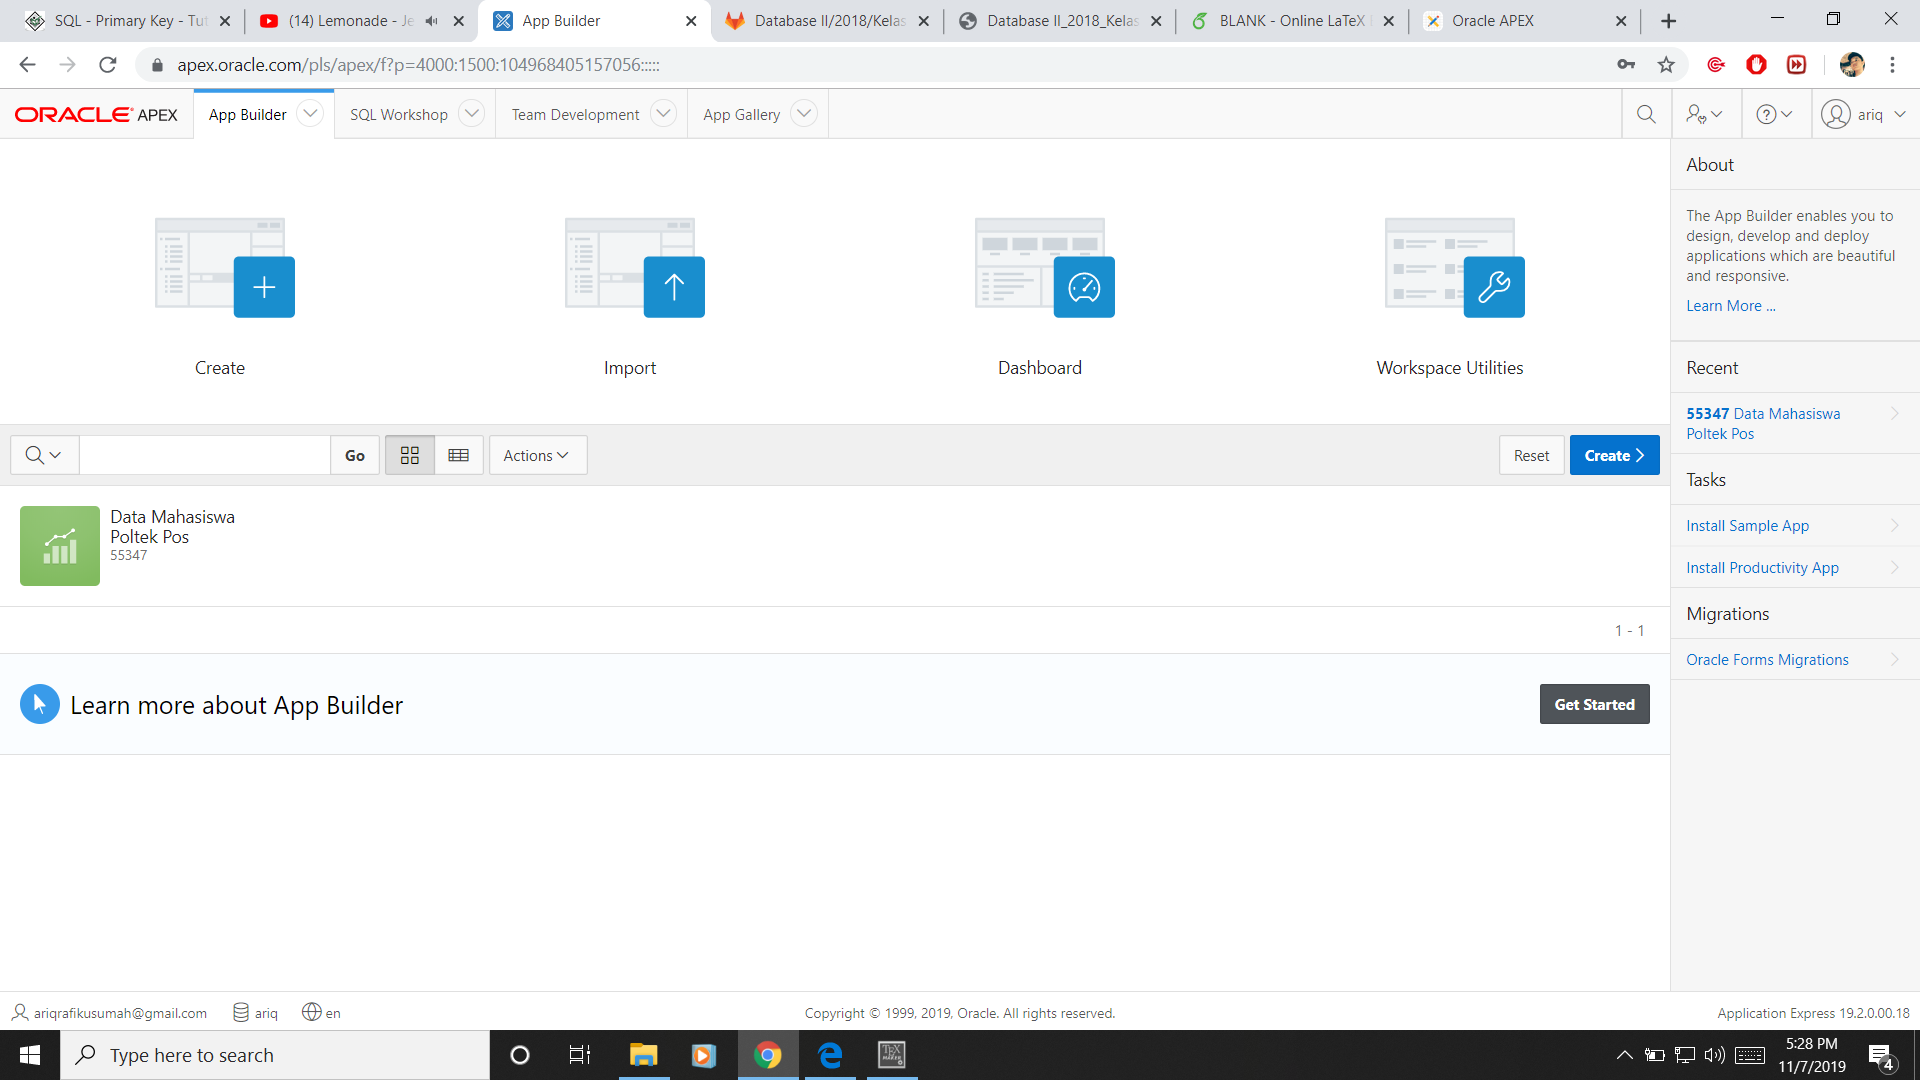
\includegraphics[scale=0.2]{Gambar/Capture1}
	\caption{Tampilan}
\end{figure}

\item Lalu lakukan Normalisasi di Excle.
\\
\\
\\
\\
\\
\\
\\
\item Masuk ke menu Create lalu Klik From a File.
\begin{figure}[h]
	\centering
		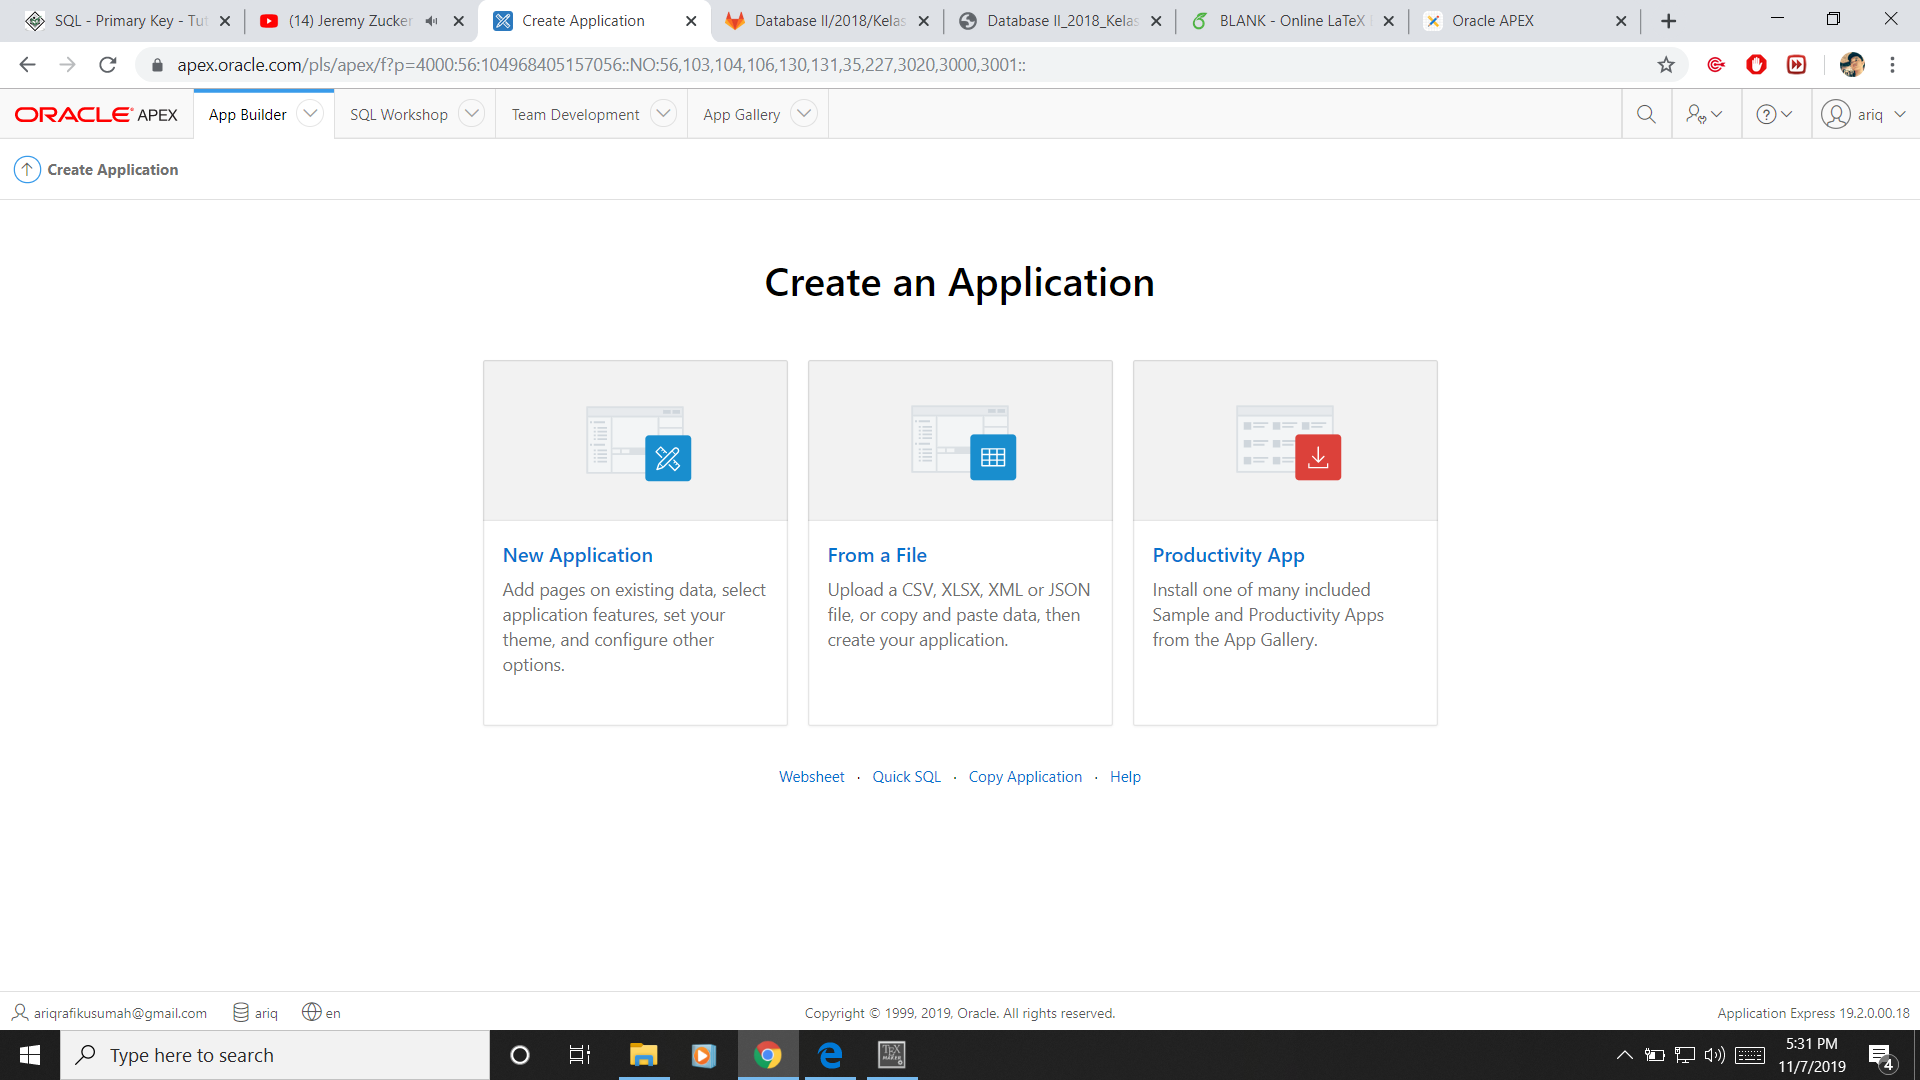
\includegraphics[scale=0.2]{Gambar/Capture2}
	\caption{From A File}
\end{figure}
\\
\\
\\
\\
\\
\item Drag and Drop file Excle yang sudah di normalisasi.
\begin{figure}[h]
	\centering 
		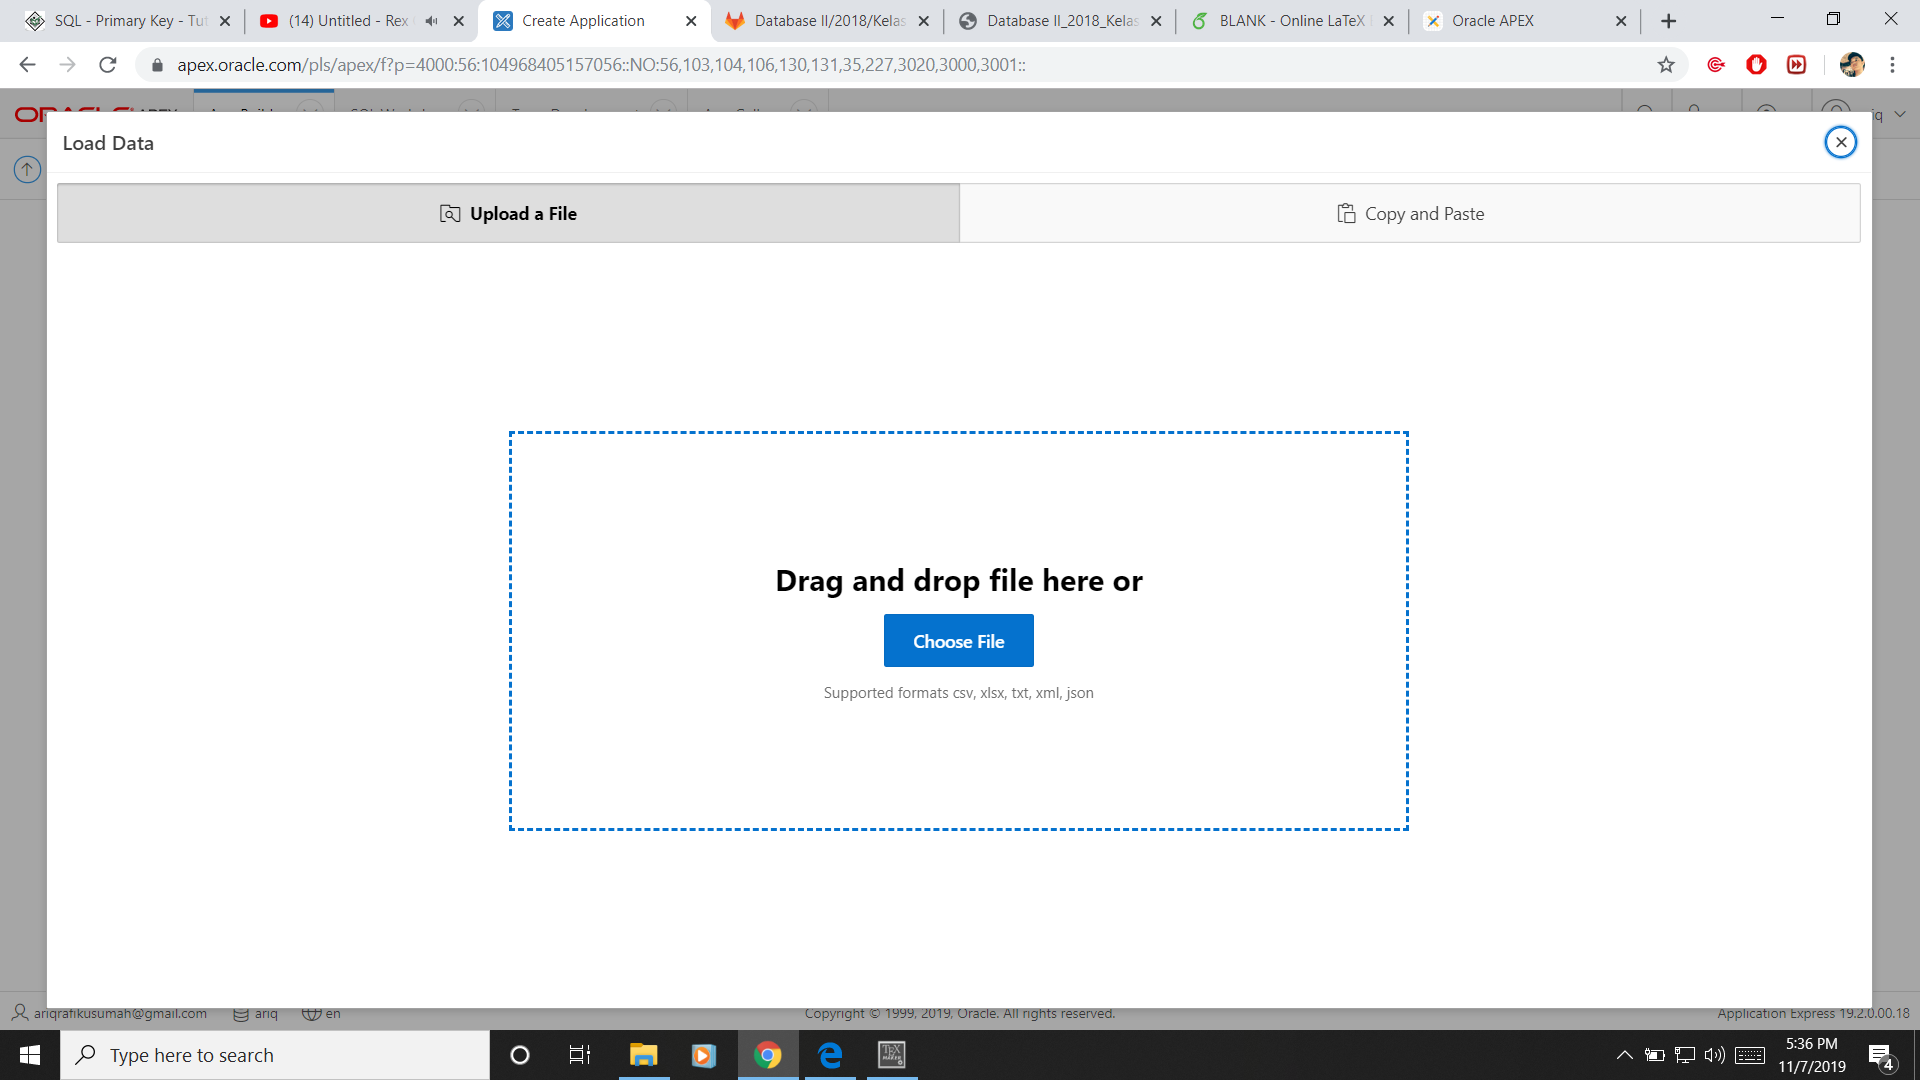
\includegraphics[scale=0.2]{Gambar/Capture3}
	\caption{Drag and Drop}
\end{figure}
\\
\\
\\
\\
\item Isikan Tabel Name dengan nama TABEL\textunderscore MAHASISWA tidak boleh menggunakan spasi.
\begin{figure}[h]
	\centering
		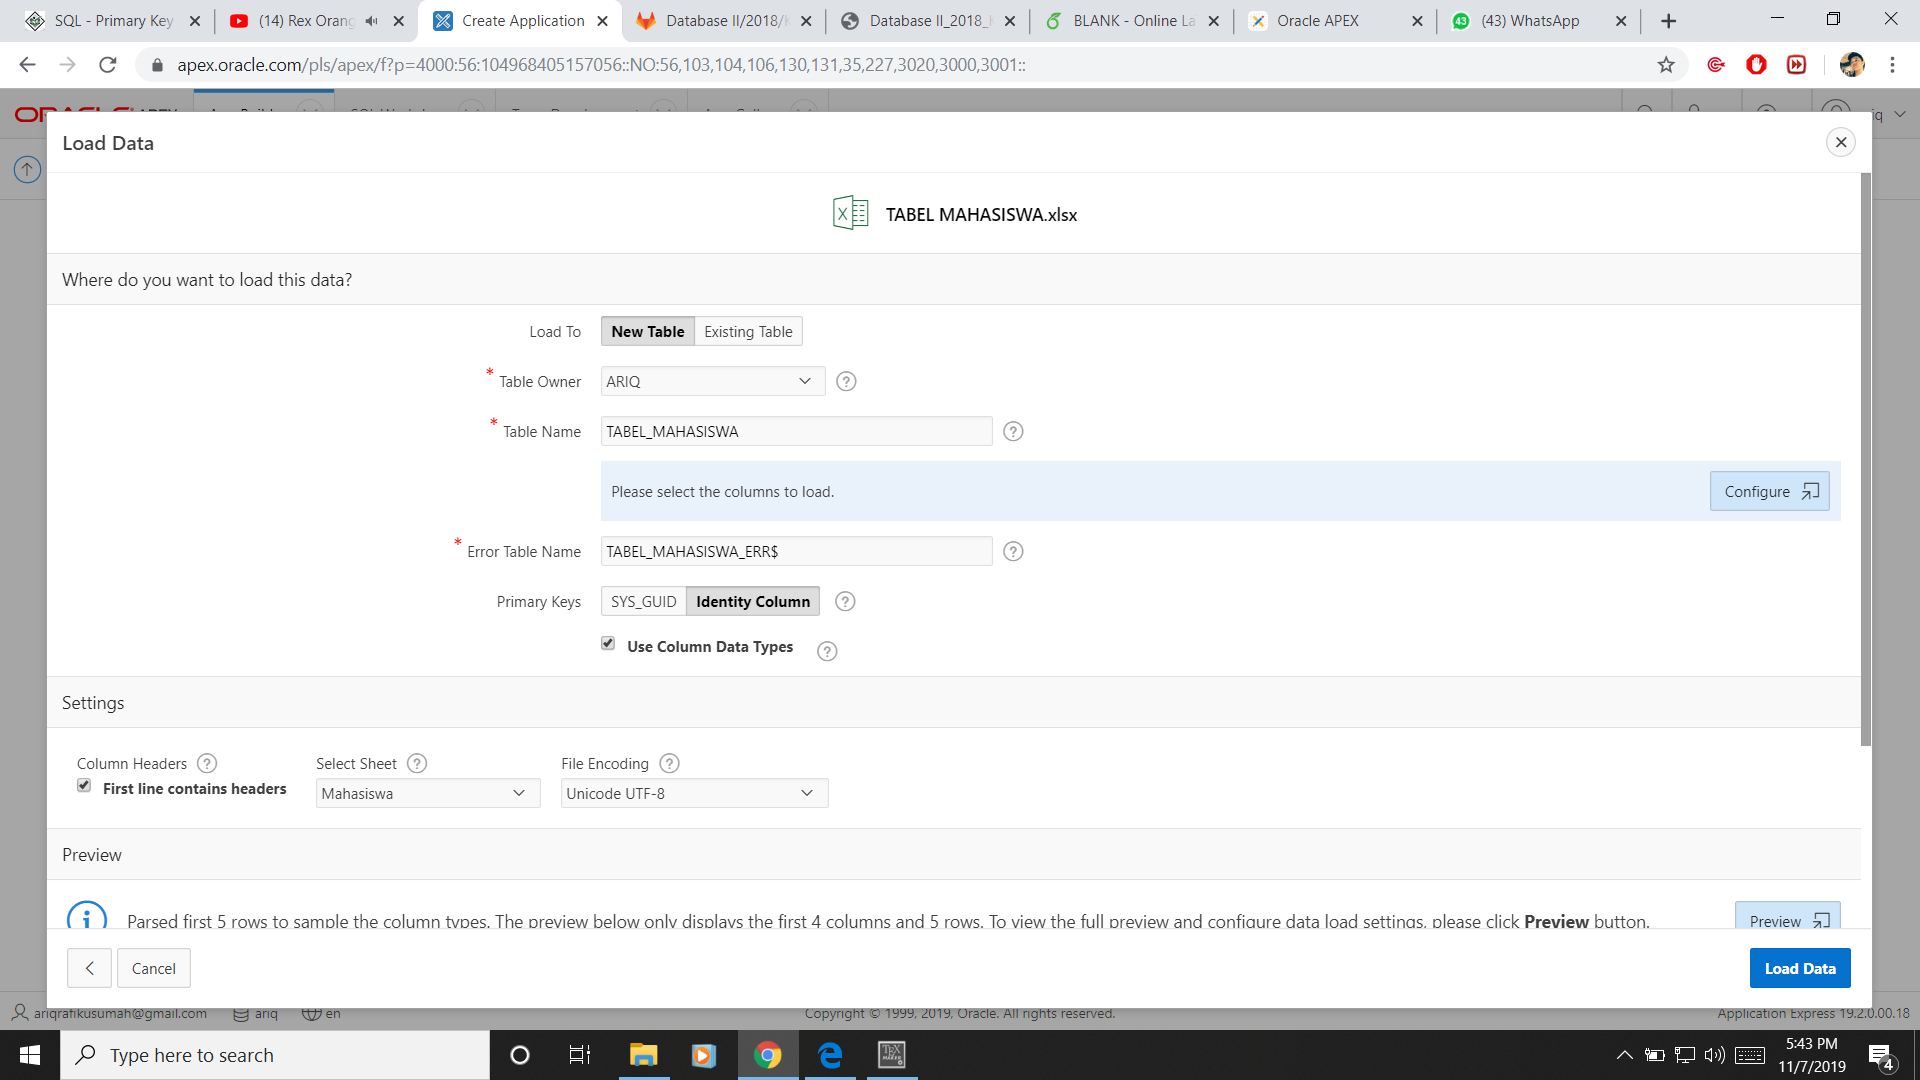
\includegraphics[scale=0.2]{Gambar/Capture4}
	\caption{Membuat Tabel}
\end{figure}[h]
\item Setelah tebuat Tabel nya jangan langsung Create Application, lalukan Pembuatan tabel sebanyak yang anda punya, dengan cara Drag and Drop lagi.
\begin{figure}[h]
	\centering
		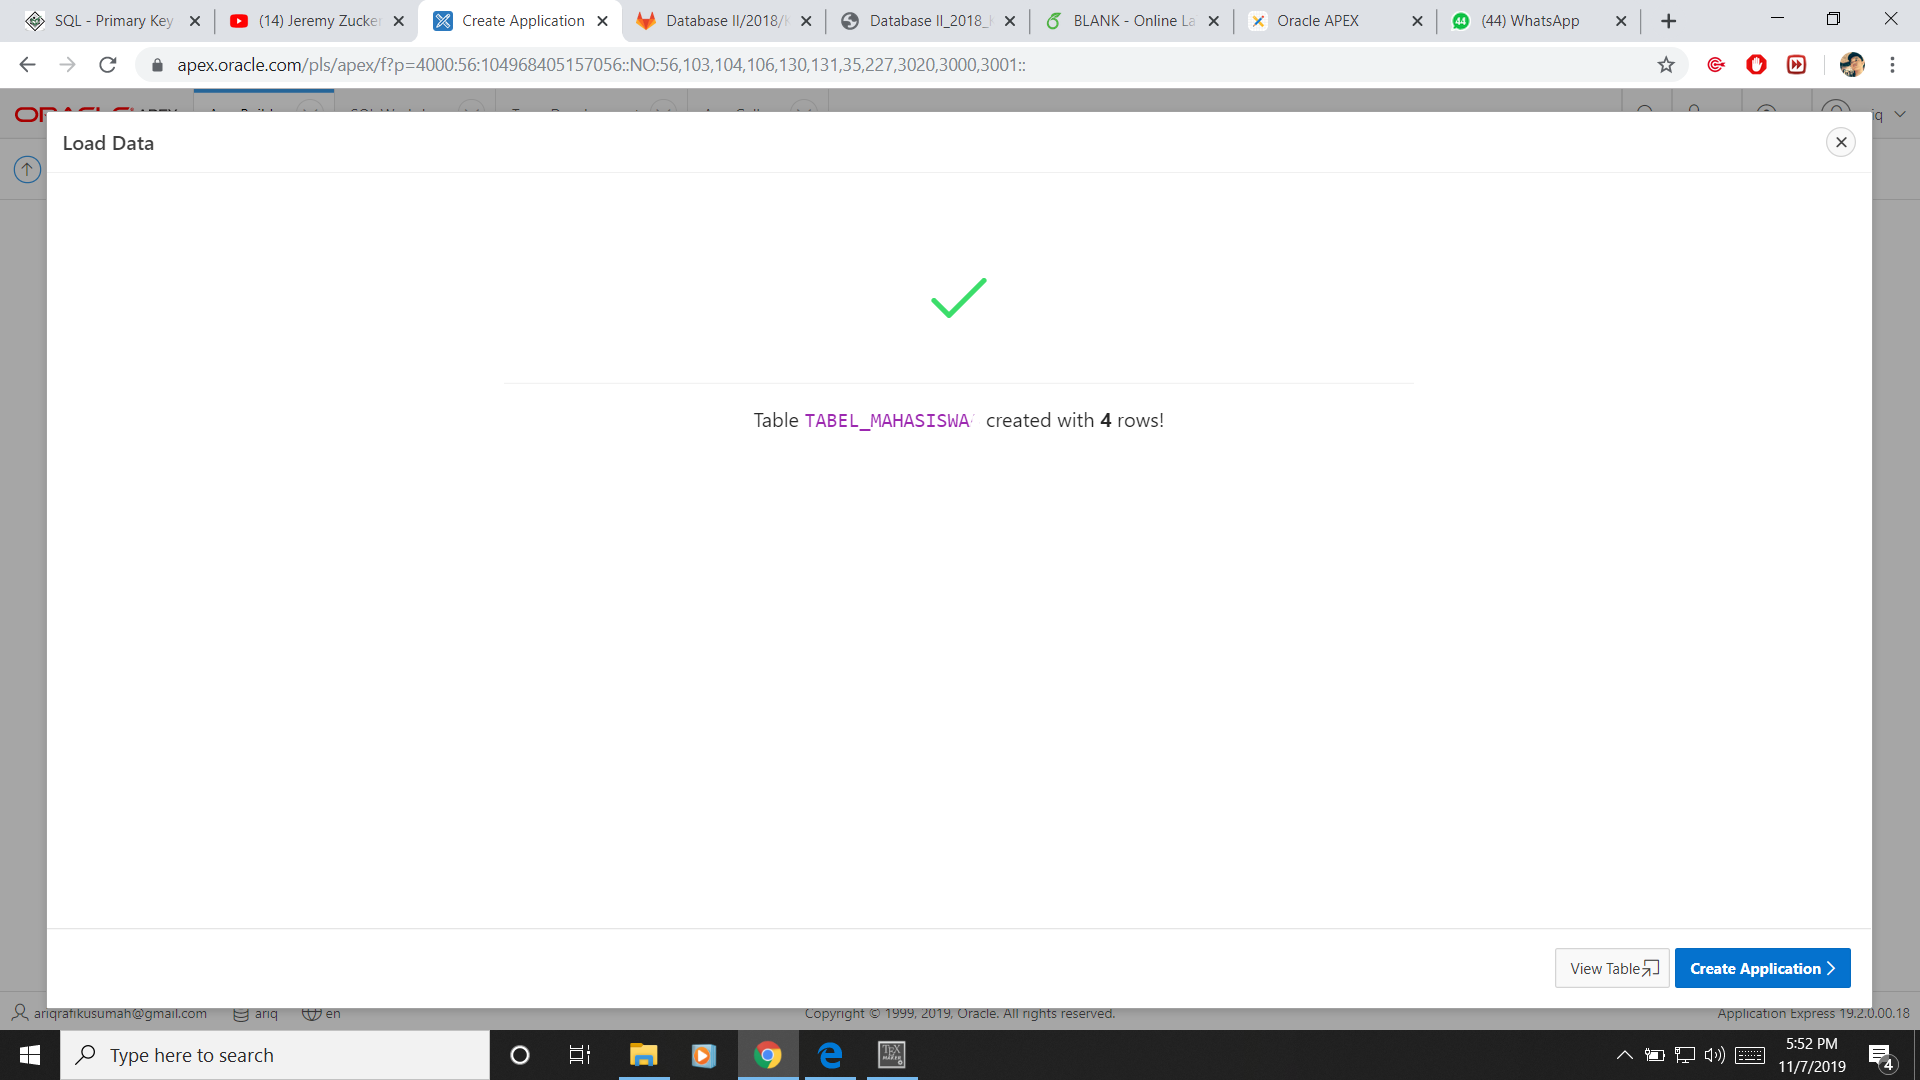
\includegraphics[scale=0.2]{Gambar/Capture5}
	\caption{Pembuatan Tabel}
\end{figure}
\\
\\
\\
\\
\\
\\
\\
\item Buka Tools Obejext Browser Untuk memastikan sudah masuk semua Tabel Sudah Masuk.

\begin{figure}[h]
	\centering
		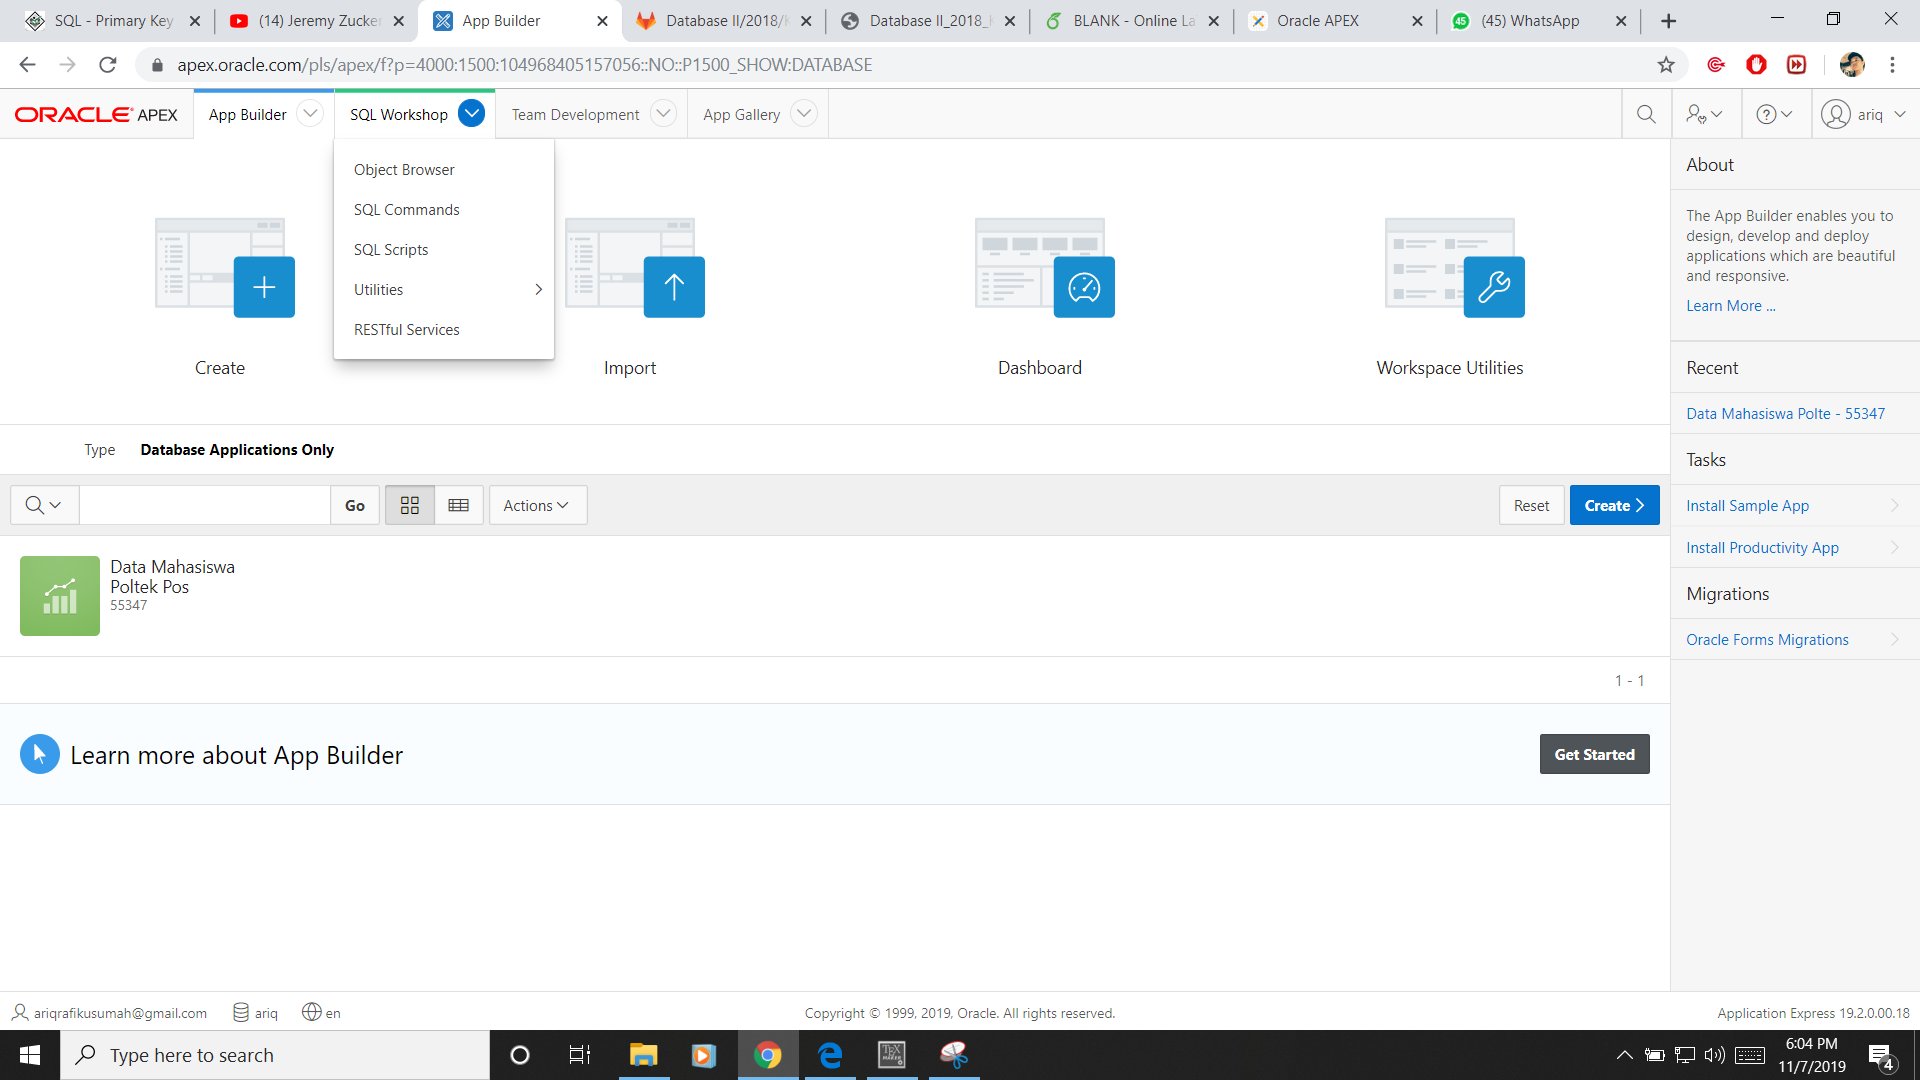
\includegraphics[scale=0.2]{Gambar/Capture6}
\end{figure}
\item Maka Akan Menampilkan seperti di bawah ini.
\begin{figure}[h]
	\centering
		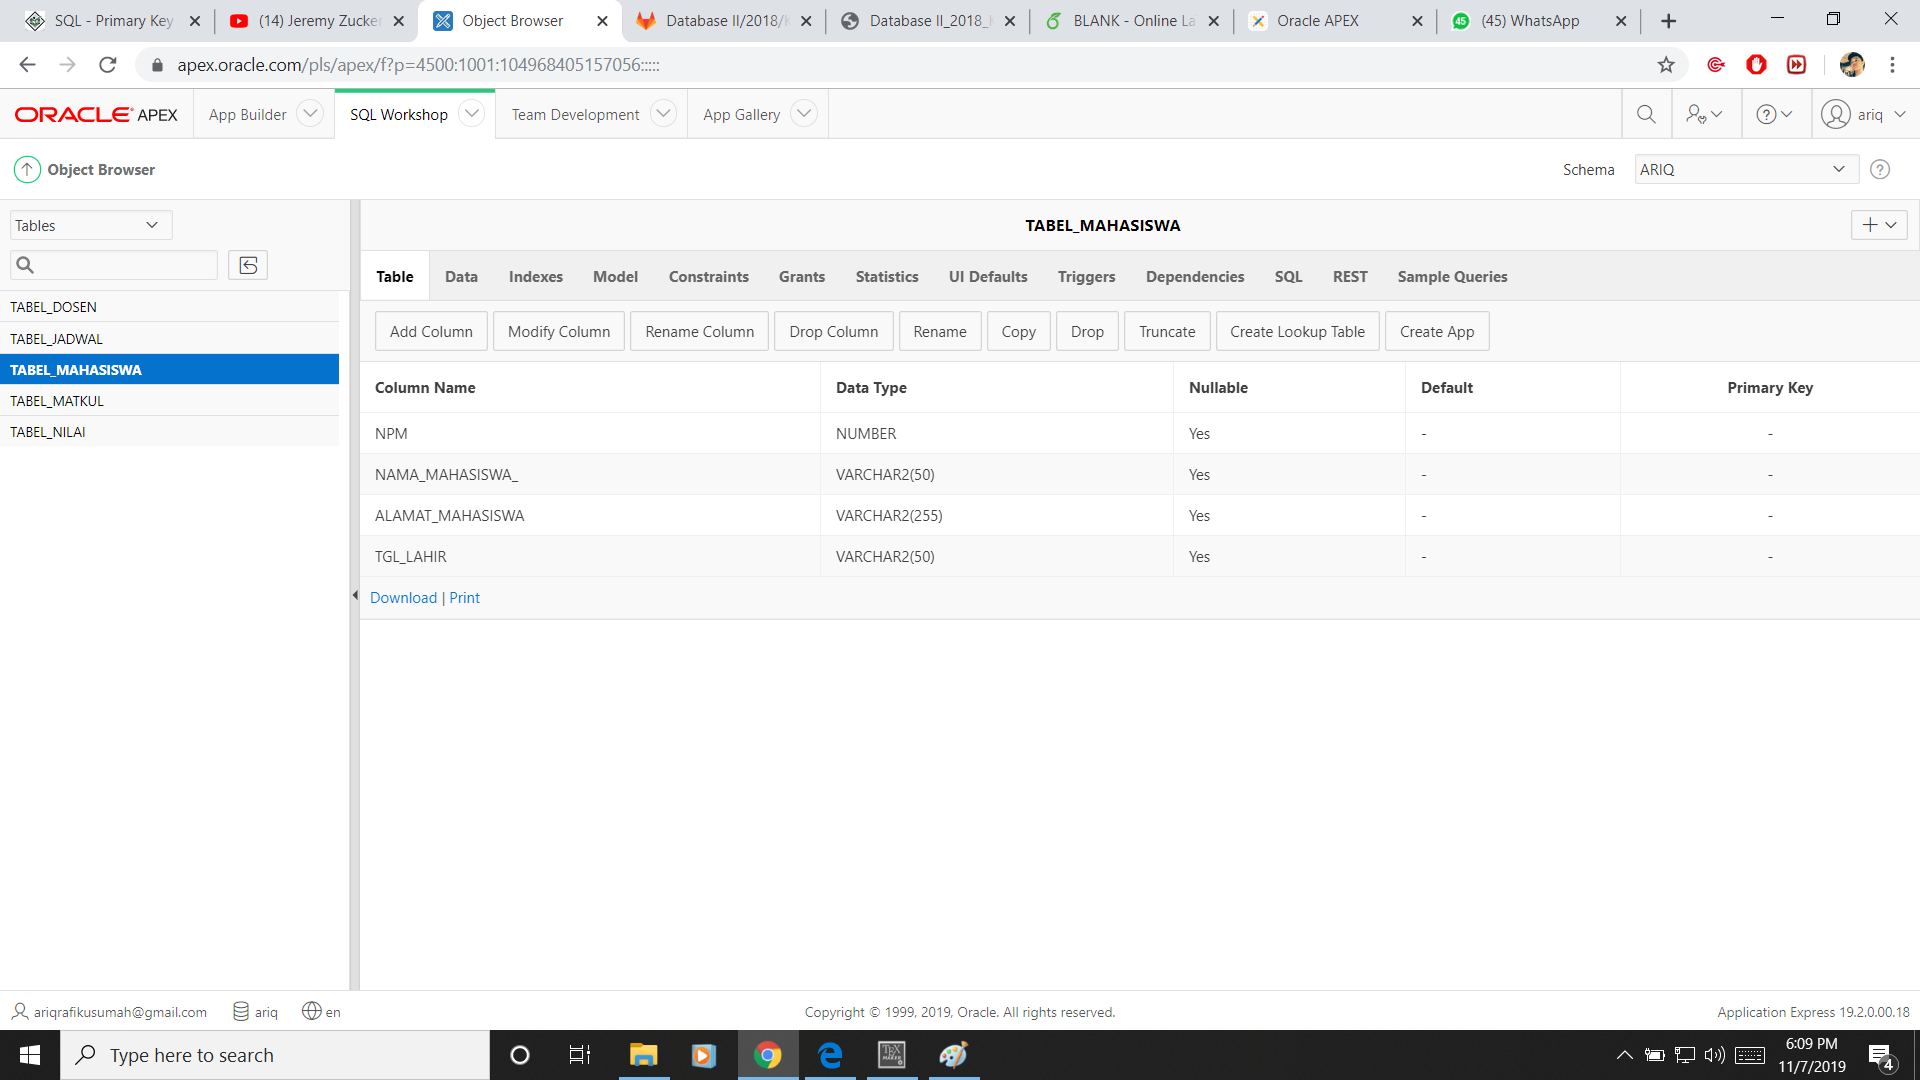
\includegraphics[scale=0.2]{Gambar/Capture7}
\end{figure}
\\
\\
\\
\\
\\
\\
\\
\\
\\
\\
\\
\\
\item Setelah Itu kita masukan primary key nya yang setiap table dengan SQL Commands.Ketikan query nya seperti di bawah ini.Lalu run tunggu samapai muncul table altered.
\begin{figure}[h]
	\centering
		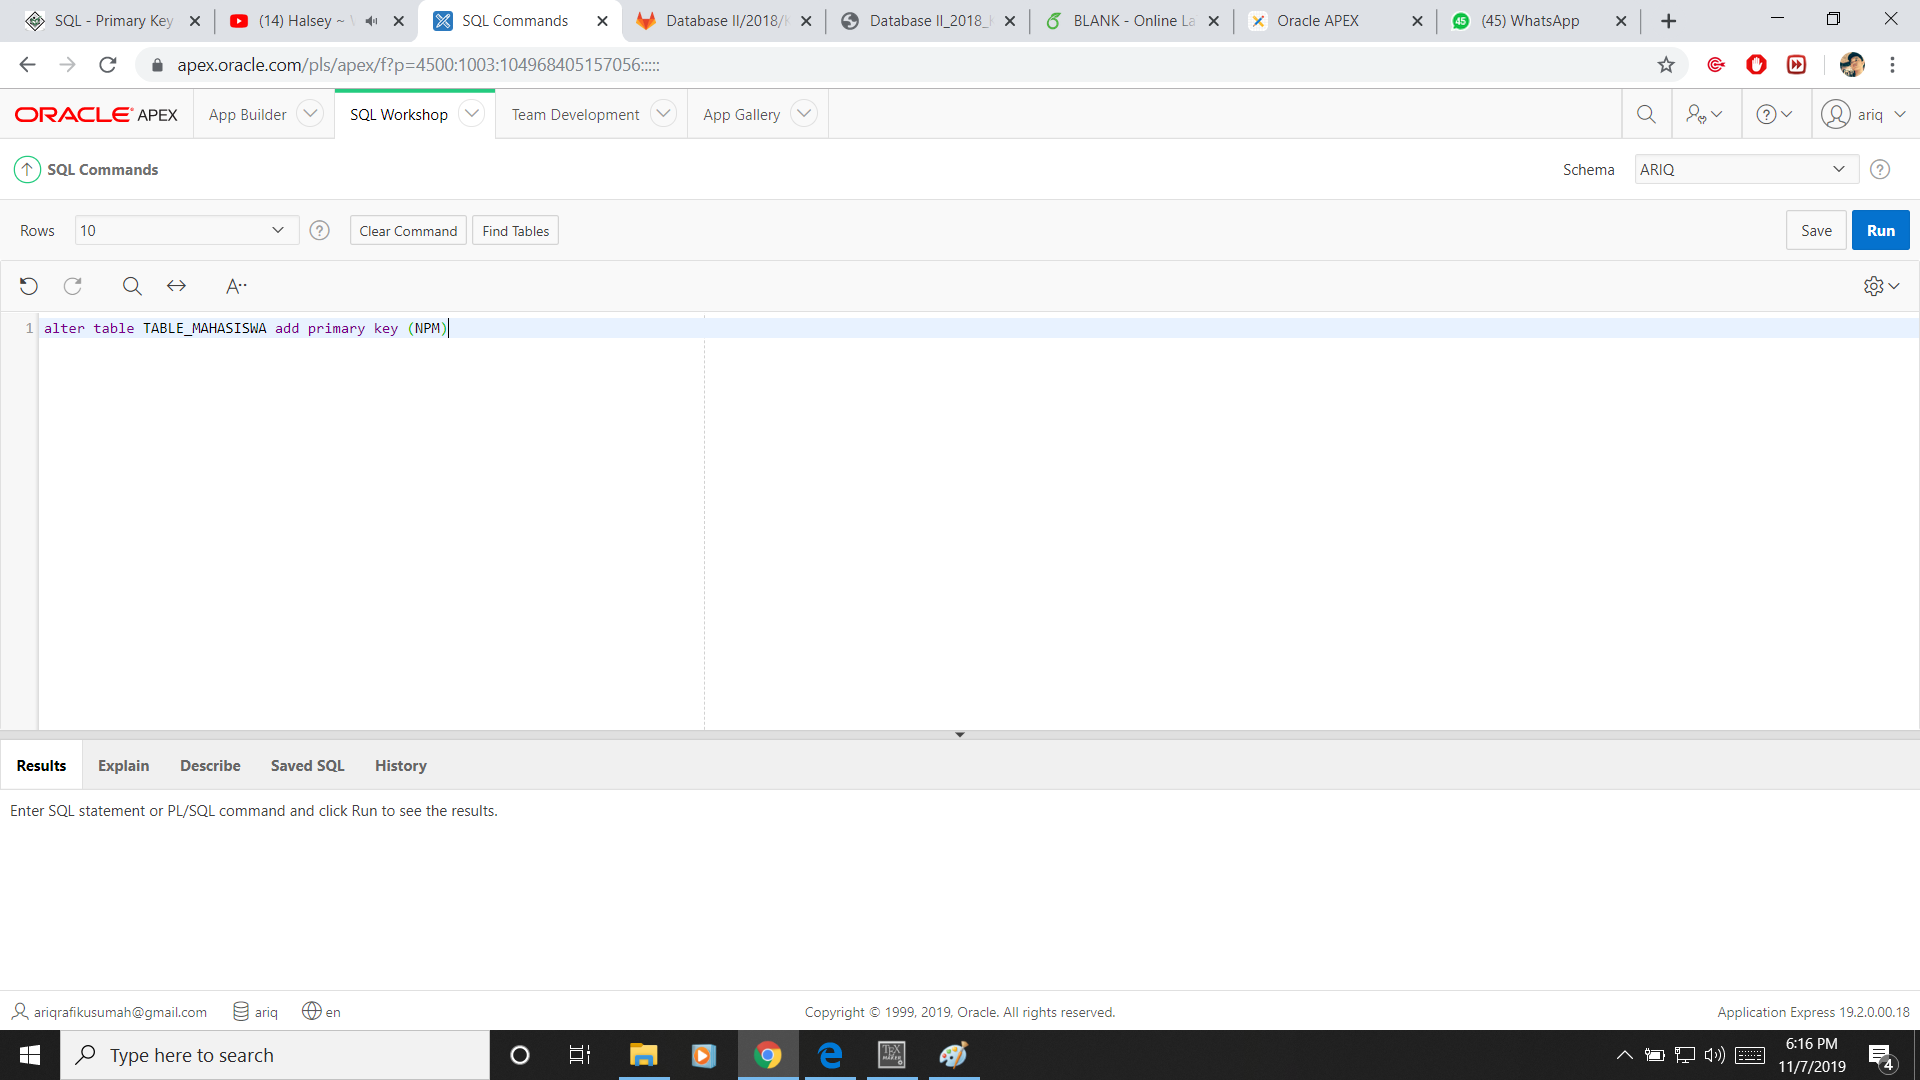
\includegraphics[scale=0.2]{Gambar/Capture8}
	\caption{SQL Commands}
\end{figure}
\item Setelah itu merelasikan tabel, mengetikan query seperti digambar.
\begin{figure}[h]
	\centering
		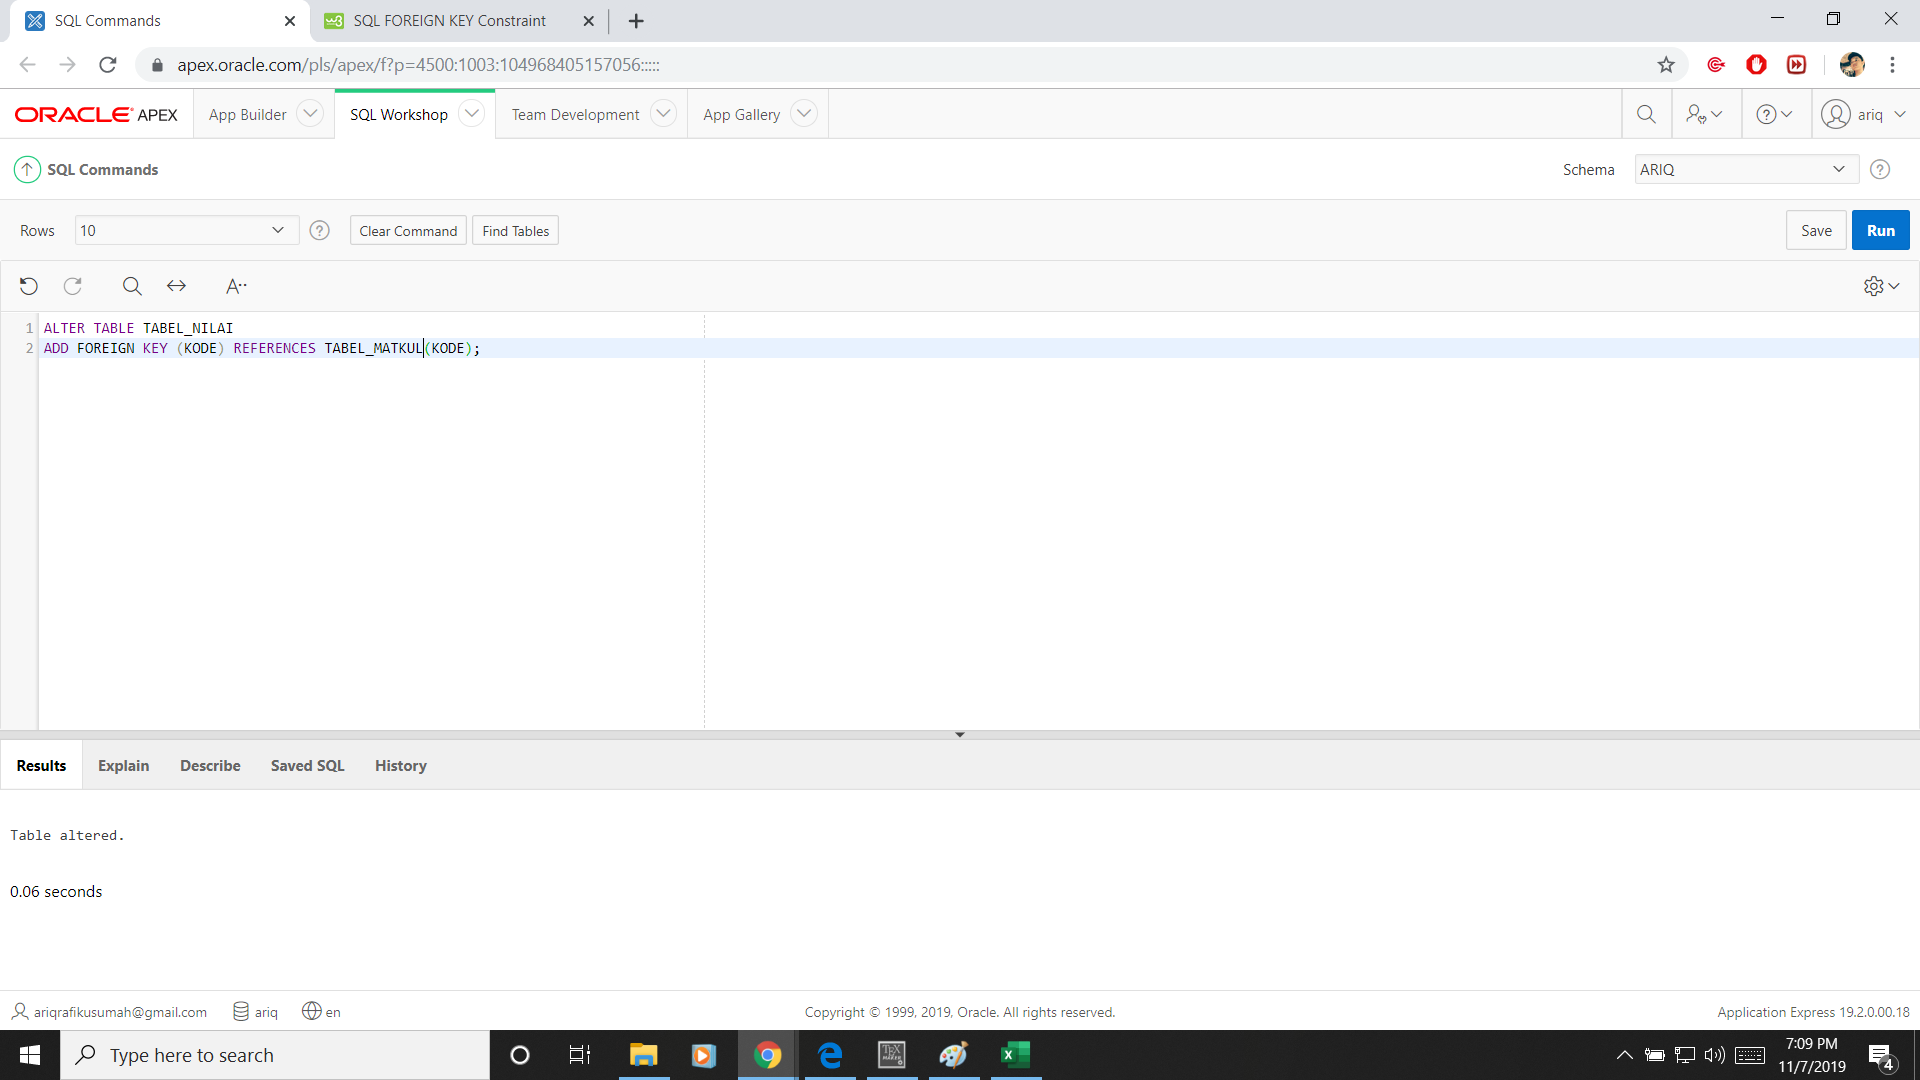
\includegraphics[scale=0.2]{Gambar/Capture9}
	\caption{Relasi}
\end{figure}
\\
\\
\\
\\
\\
\\
\\
\\
\item Setelah Tabel berelasi , Langkah selanjutnya membuat application 

\begin{figure}[h]
	\centering
		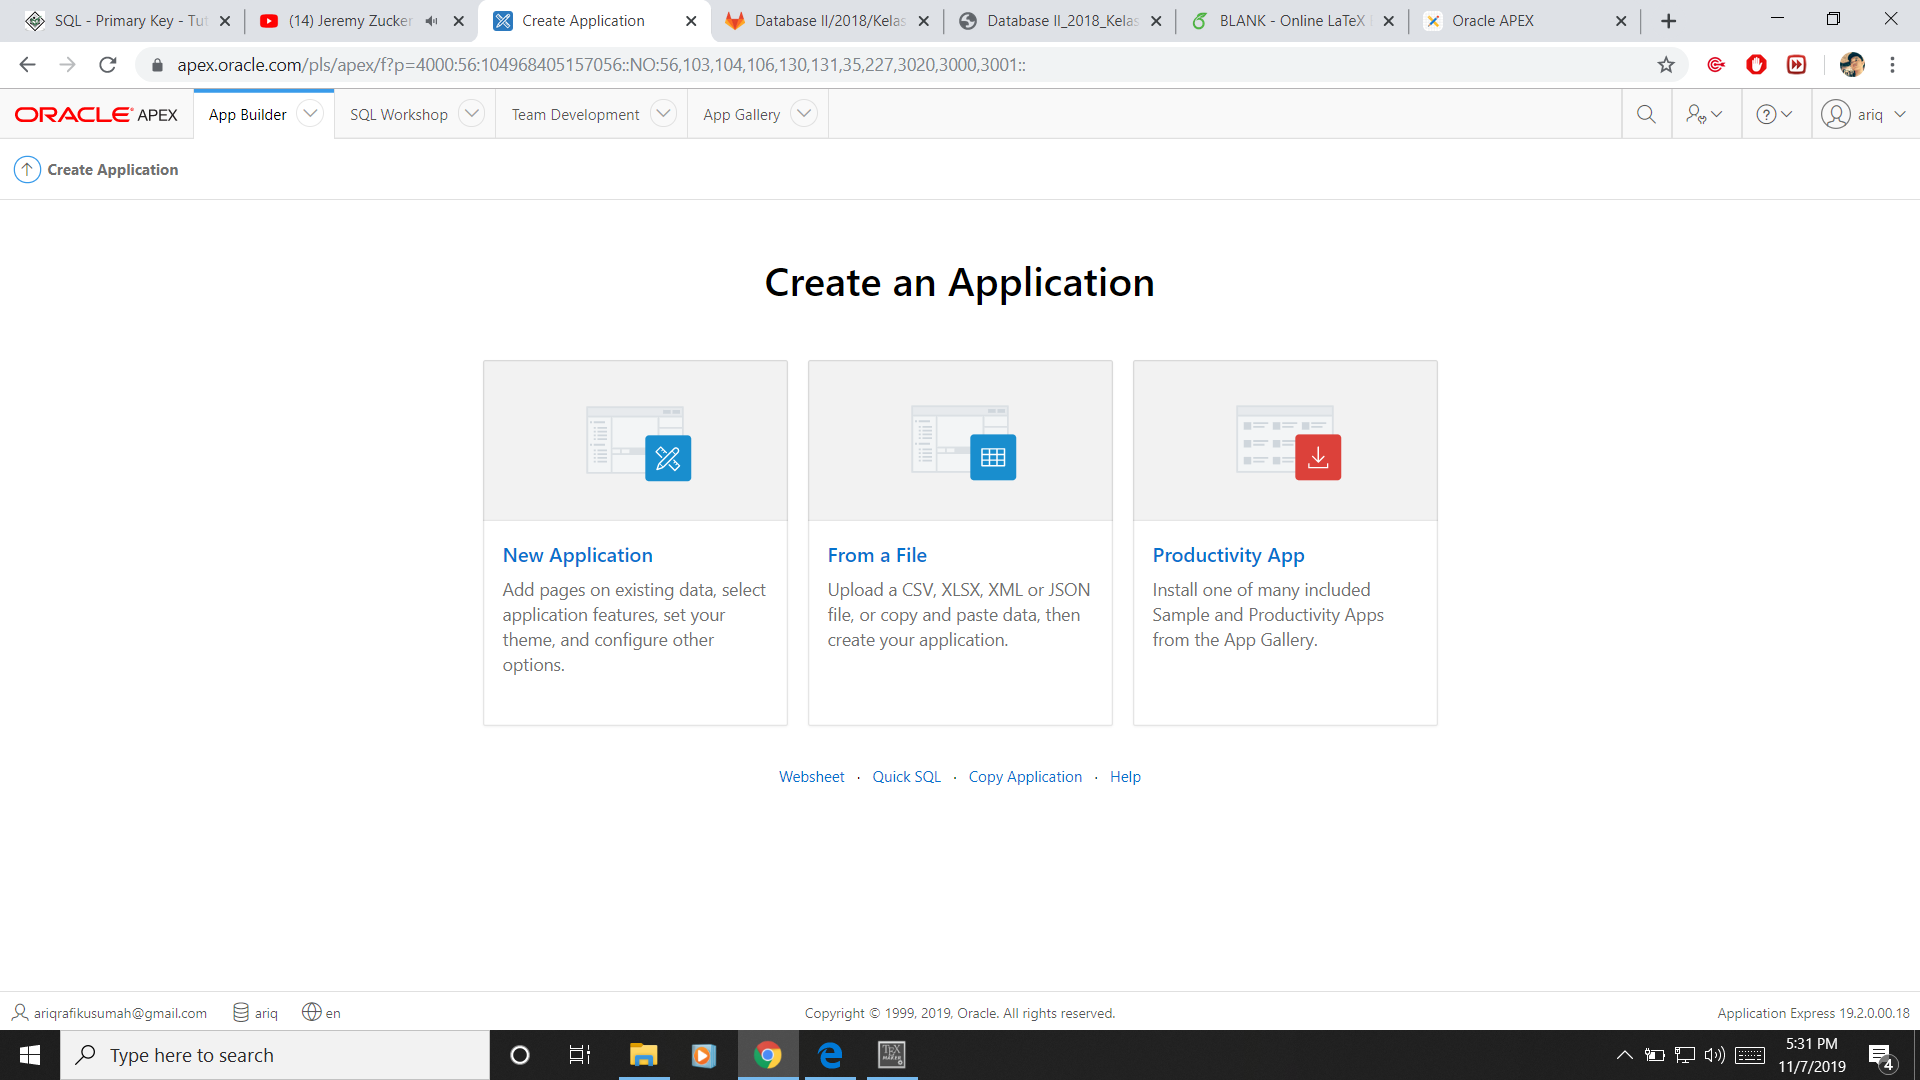
\includegraphics[scale=0.2]{Gambar/Capture2}
	\caption{Create App}
\end{figure}

\item Klik pada menu New Application, Lalu isikan Nama, dan klik pada Add Page
\begin{figure}[h]
	\centering
		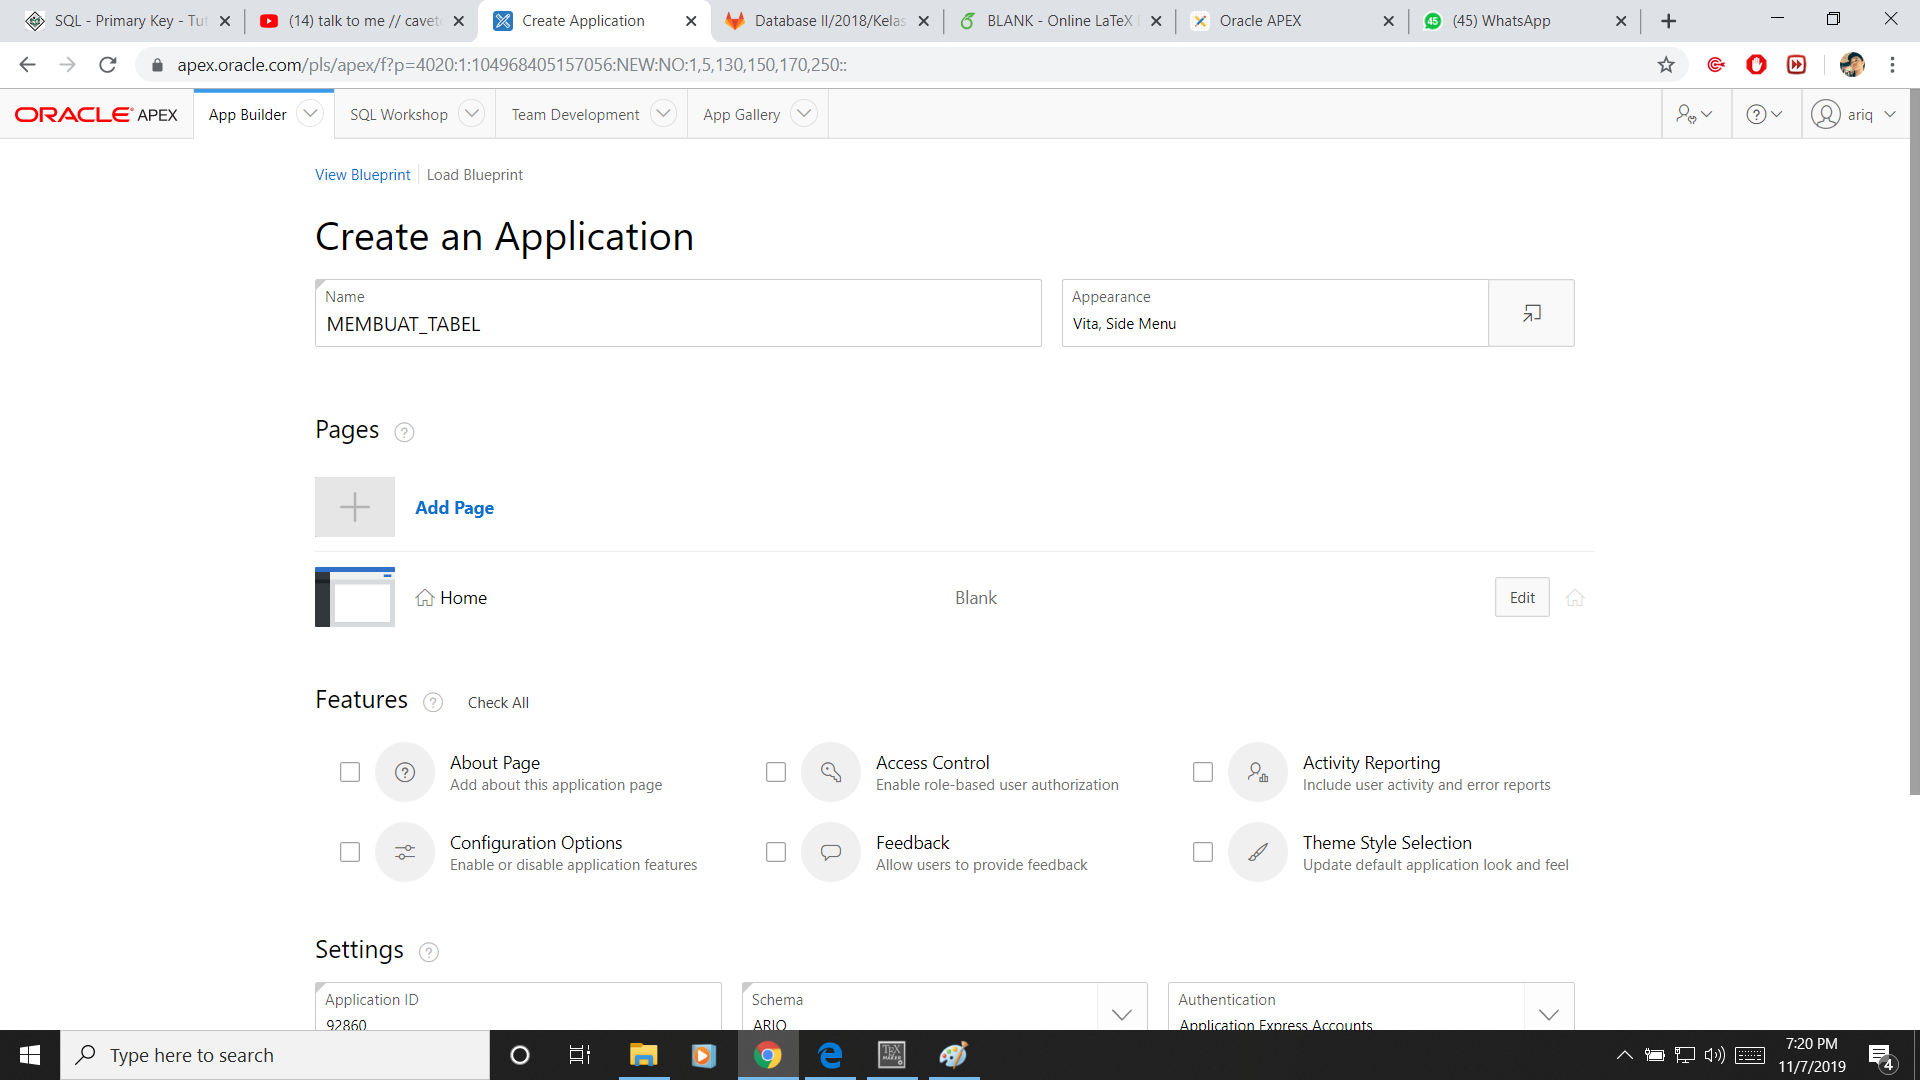
\includegraphics[scale=0.2]{Gambar/Capture10}
\end{figure}
\\
\\
\\
\\
\\
\\
\\
\\
\\
\\
\\
\\
\item Pilih Page \textbf{Interactive Report}.
\begin{figure}[h]
	\centering
		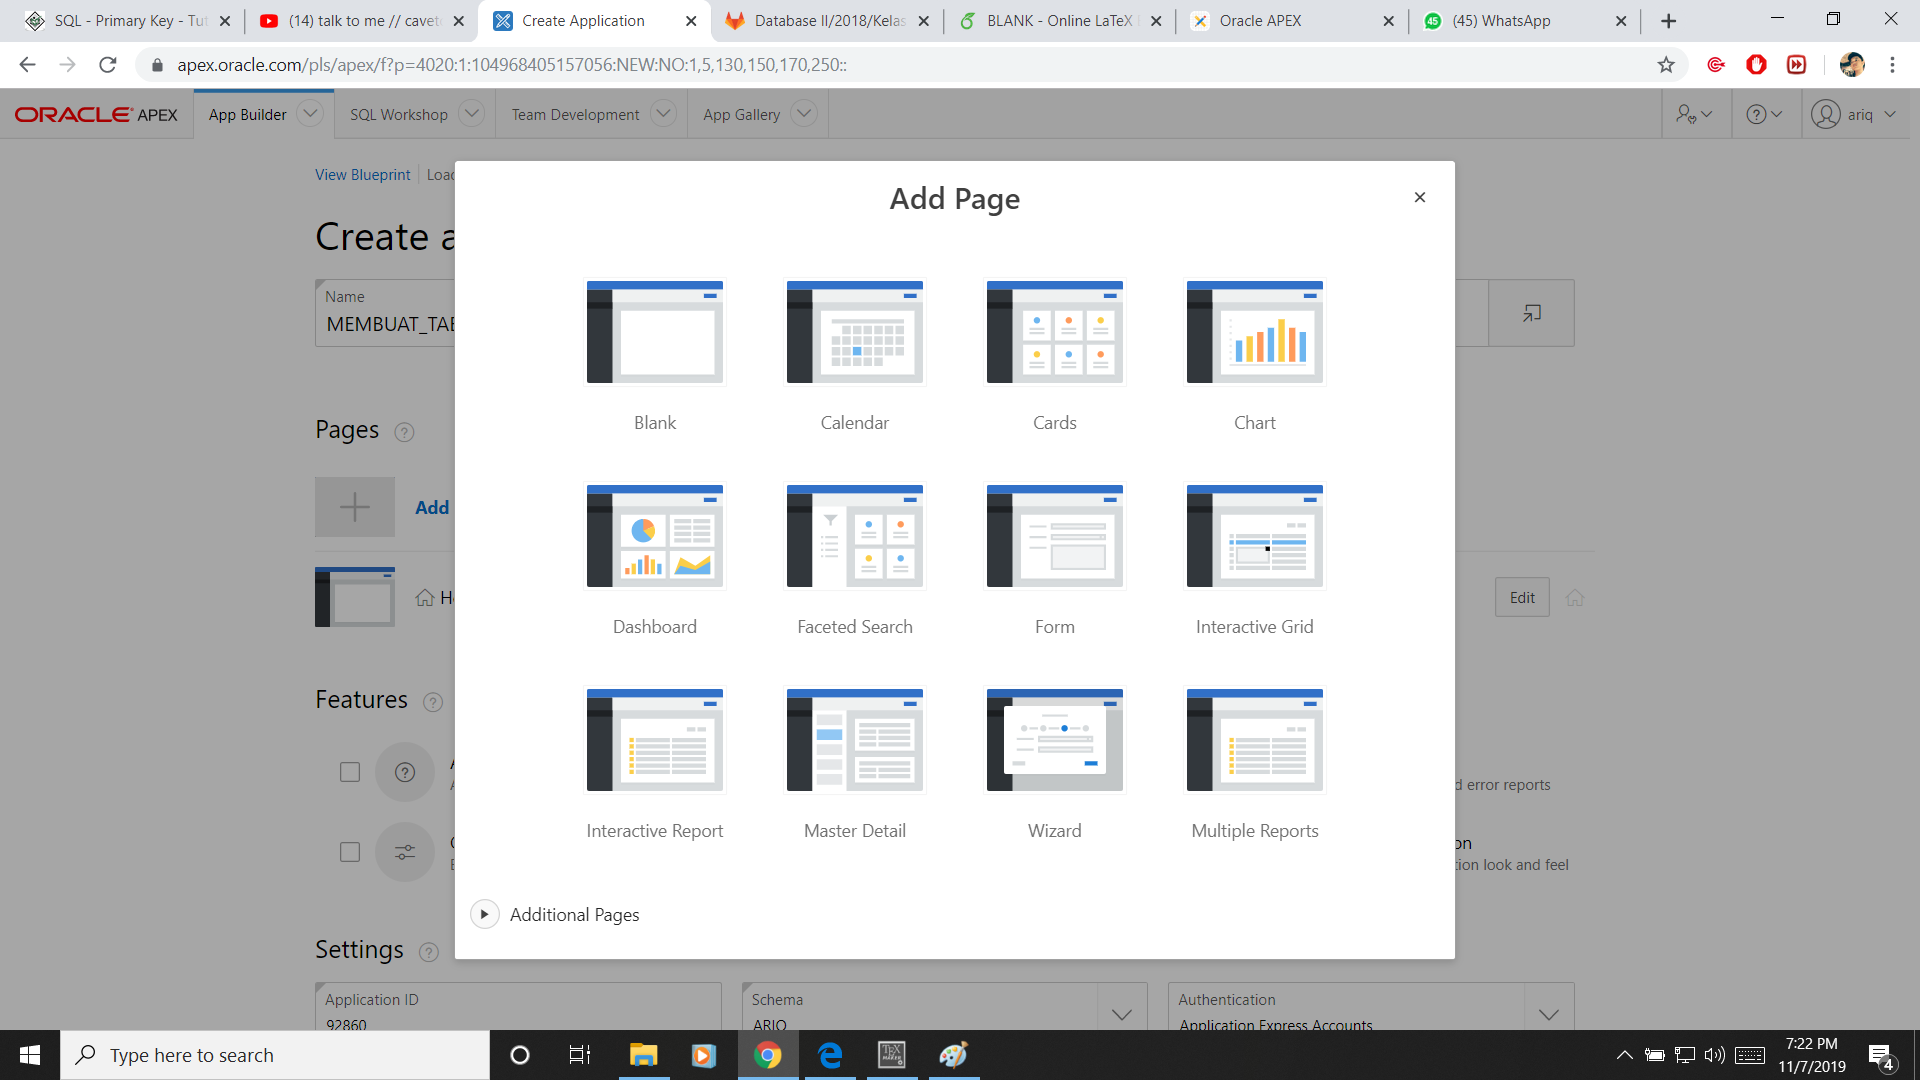
\includegraphics[scale=0.2]{Gambar/Capture11}
	\caption{Page Option}
\end{figure}
\item Isikan nama Pagenya, dan table nya yang dipilih sesuai ingin di tampilkan, lalu add page.
\begin{figure}[h]
	\centering
		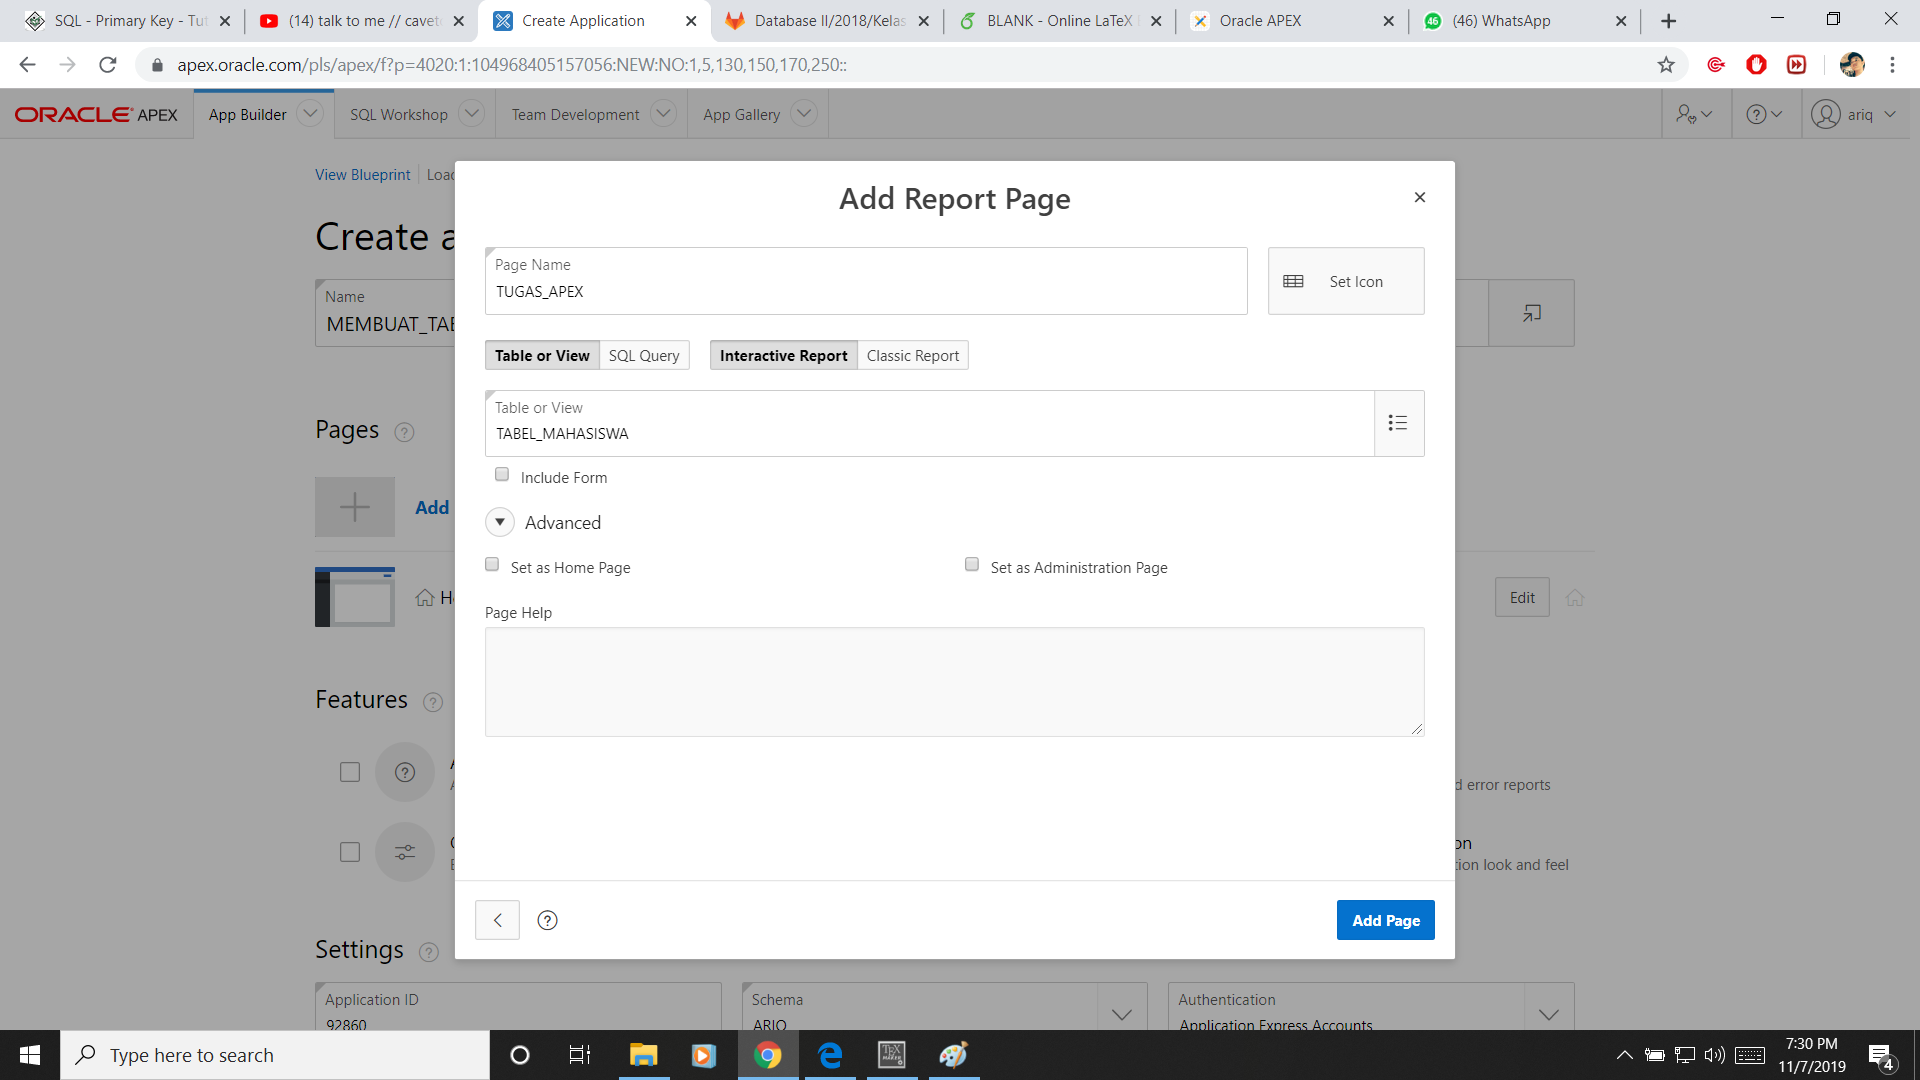
\includegraphics[scale=0.2]{Gambar/Capture12}
	\caption{Membuat tabel page}
\end{figure}
\\
\\
\\
\\
\\
\\
\\
\\
\\
\item Scroll Kebawah, Setelah itu Create Application, Lalu Run Application.

\begin{figure}[h]
	\centering
		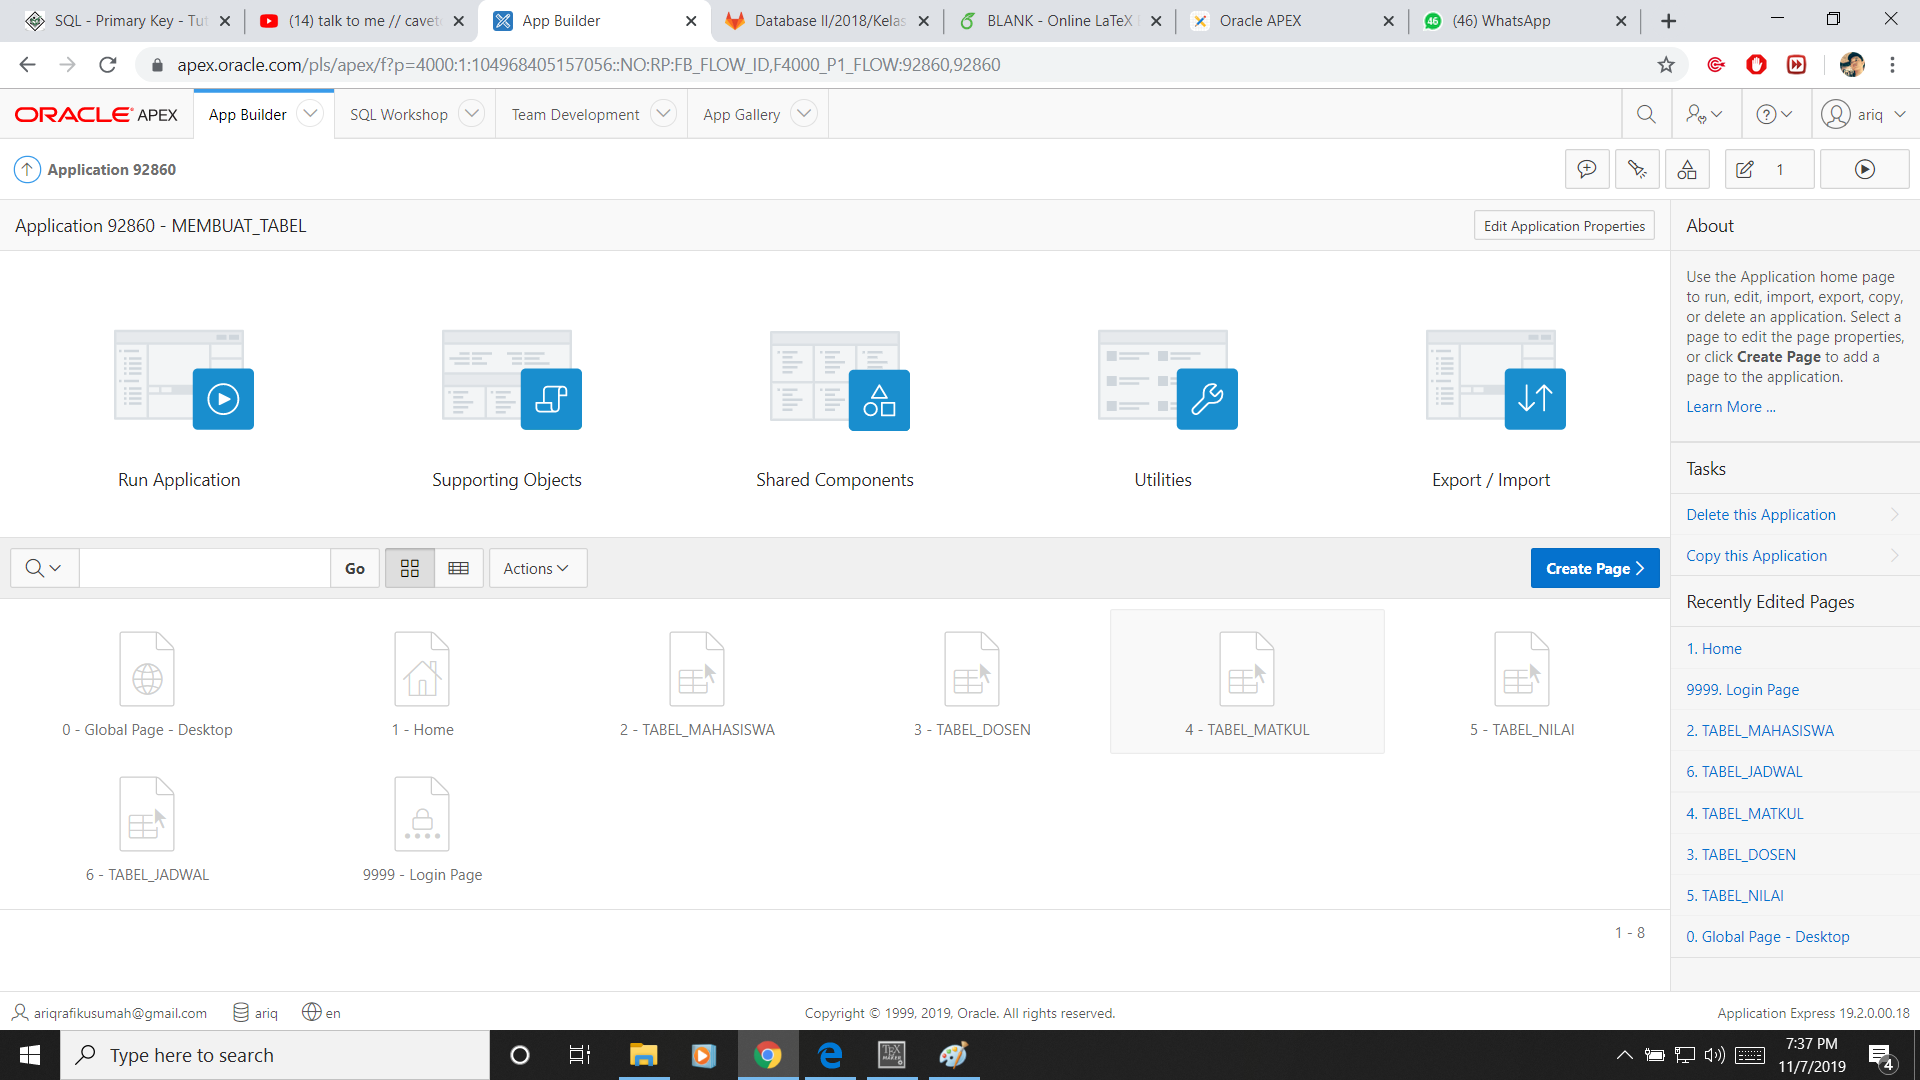
\includegraphics[scale=0.2]{Gambar/Capture13}
	\caption{Run App}
\end{figure}
\item Maka akan menampilkan seperti di bawah ini :
\begin{figure}[h]
	\centering
		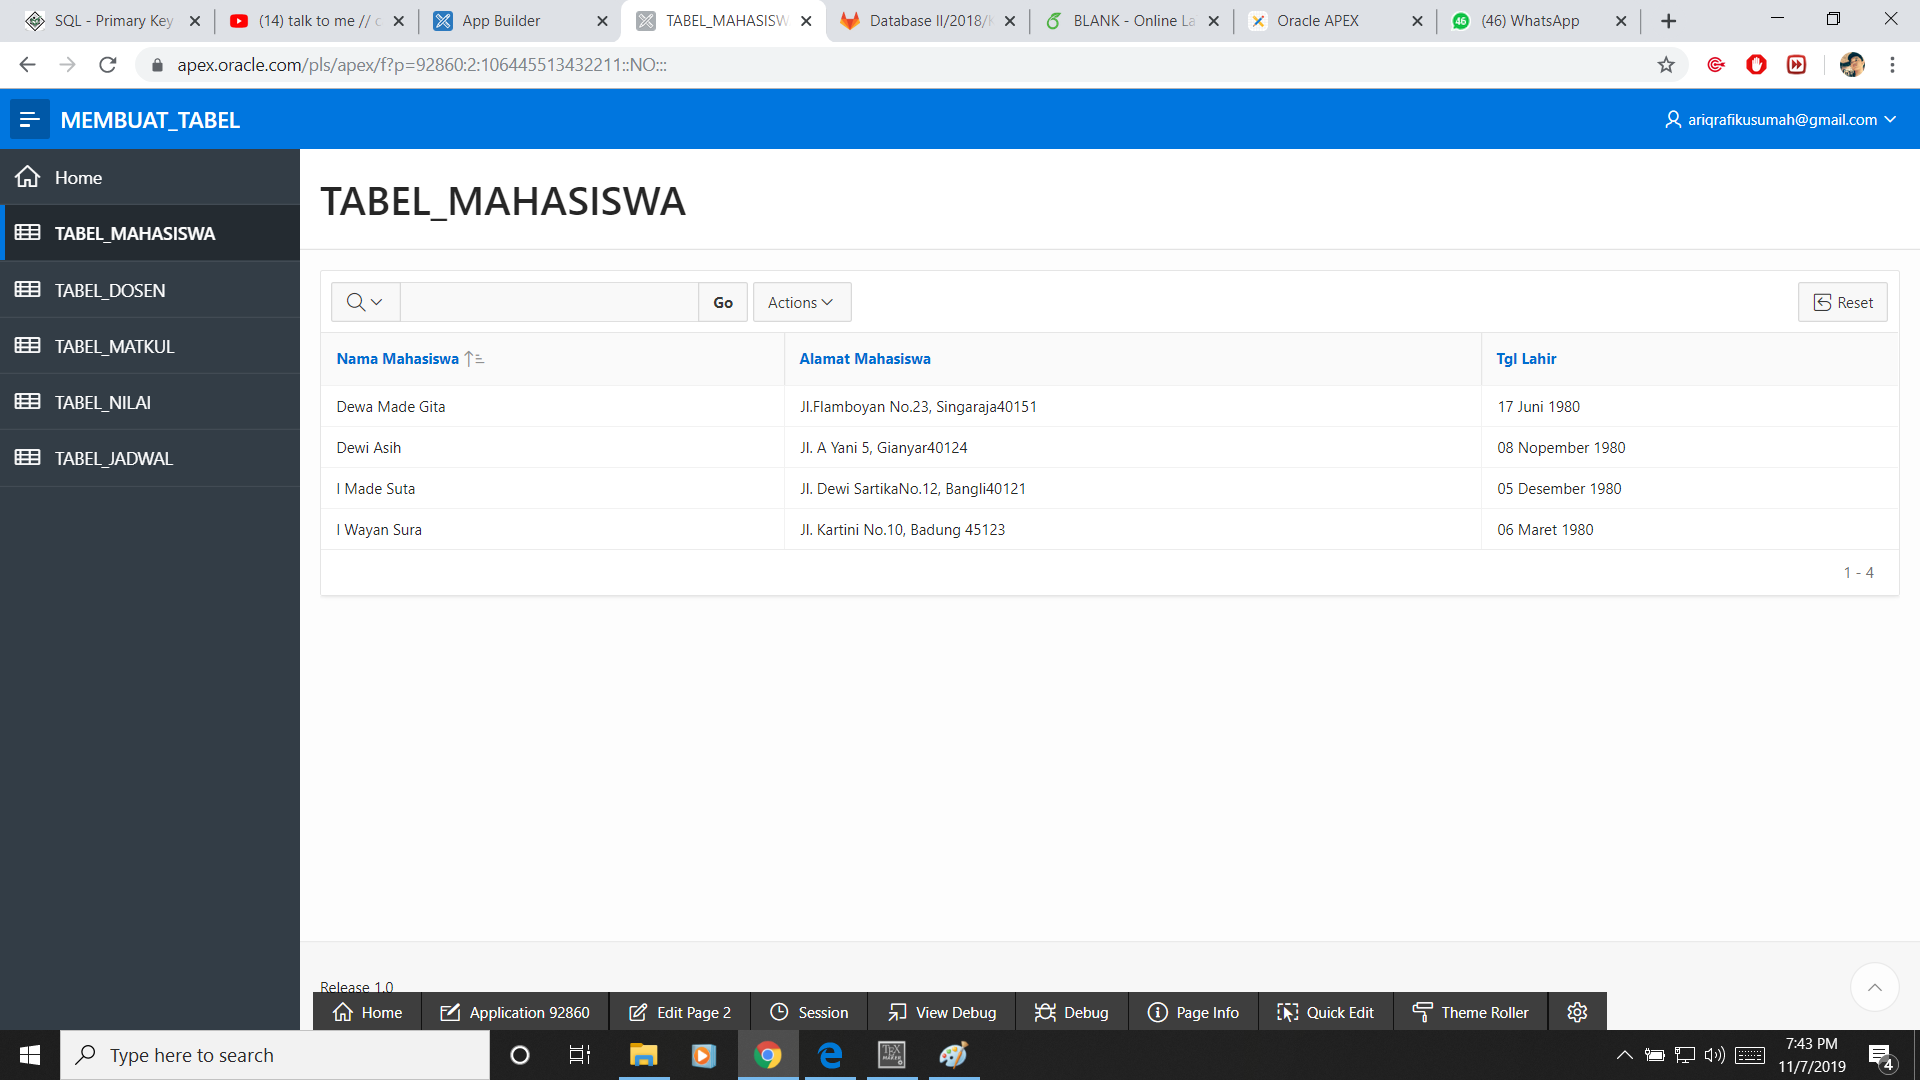
\includegraphics[scale=0.3]{Gambar/Capture14}
	\caption{CONTOH}
\end{figure}
\\
\\
\\
\\
\section{LOGIN ORACLE APEX}
\subsection{USERNAME, PASSWORD dan LINK}
\begin{enumerate}
\item workspace \textbf{ariq}
\item username  \textbf{ariqrafikusumah@gmail.com}
\item password  \textbf{ariq021336699}
\item Link		 \textbf{https://apex.oracle.com/pls/apex/f?p=92860:LOGIN\textunderscore DESKTOP:\\713112418532266:::::}

\end{enumerate}
\end{enumerate}
\end{document}
